\documentclass[11pt,a4paper]{report}
\usepackage[portuges]{babel}
\usepackage[utf8]{inputenc} % define o encoding usado texto fonte (input)--usual "utf8" ou "latin1
\usepackage{graphicx} %permite incluir graficos, tabelas, figuras
\usepackage{subcaption}
\usepackage{listings}
\usepackage{color}
\usepackage{multicol}
\usepackage{indentfirst}
\usepackage{hyperref}
\usepackage{amsmath}
\usepackage{amssymb}
\usepackage{float}
\usepackage{enumitem}
\usepackage{tabularx}
\usepackage{atbegshi}
\parskip=2pt % espaço entre o parágrafo e o texto anterior

\setlength{\oddsidemargin}{-1cm} %espaço entre o texto e a margem
\setlength{\textwidth}{18cm} %Comprimento do texto na pagina
\setlength{\headsep}{-1cm} %espaço entre o texto e o cabeçalho
\setlength{\textheight}{23cm} %altura do texto na pagina


\definecolor{myblue}{rgb}{0.2,0.2,0.8}
\definecolor{mygray}{rgb}{0.5,0.5,0.5}
\definecolor{mymauve}{rgb}{0.58,0,0.82}

\lstdefinestyle{code}{ 
  backgroundcolor=\color{white},   % choose the background color; you must add \usepackage{color} or \usepackage{xcolor}; should come as last argument
  basicstyle=\footnotesize,        % the size of the fonts that are used for the code
  breakatwhitespace=false,         % sets if automatic breaks should only happen at whitespace
  breaklines=true,                 % sets automatic line breaking
  captionpos=b,                    % sets the caption-position to bottom
  commentstyle=\color{white},    % comment style
  deletekeywords={...},            % if you want to delete keywords from the given language
  escapeinside={\%*}{*)},          % if you want to add LaTeX within your code
  extendedchars=true,              % lets you use non-ASCII characters; for 8-bits encodings only, does not work with UTF-8
  firstnumber=1000,                % start line enumeration with line 1
  keepspaces=true,                 % keeps spaces in text, useful for keeping indentation of code (possibly needs columns=flexible)
  keywordstyle=\color{blue},       % keyword style
  language=C++,                 % the language of the code
  morekeywords={*,...},            % if you want to add more keywords to the set
  numberstyle=\tiny\color{mygray}, % the style that is used for the line-numbers
  rulecolor=\color{black},         % if not set, the frame-color may be changed on line-breaks within not-black text (e.g. comments (green here))
  showspaces=false,                % show spaces everywhere adding particular underscores; it overrides 'showstringspaces'
  showstringspaces=false,          % underline spaces within strings only
  showtabs=false,                  % show tabs within strings adding particular underscores
  stepnumber=2,                    % the step between two line-numbers. If it's 1, each line will be numbered
  stringstyle=\color{mymauve},     % string literal style
  tabsize=2,                     % sets default tabsize to 2 spaces
  title=\lstname                   % show the filename of files included with \lstinputlisting; also try caption instead of title
}

\AtBeginDocument{\AtBeginShipoutNext{\AtBeginShipoutDiscard}}

\title{Projeto - ComputationalMind\\ Desafios para Desenvolvimento  Computacional} %Titulo do documento

\author{Inês Pires Presa (A90355)\and Ivo Miguel Gomes Lima (A90214)\and Tiago André Oliveira Leite (A91693)\and Tiago dos Santos Silva Peixoto Carriço (A91695)} %autores do documento

\date{\today} %data

\begin{document}
\pagenumbering{gobble}
\clearpage
\thispagestyle{empty}

  \begin{minipage}{0.9\linewidth}
        \centering
    
\includegraphics[width=0.4\textwidth]{um.jpeg}\par\vspace{1cm}
                \href{https://www.uminho.pt/PT}
    {\scshape\LARGE Universidade do Minho} \par
    \vspace{0.6cm}
                \href{https://lcc.di.uminho.pt}
    {\scshape\Large Licenciatura em Ciências da Computação} \par
    \maketitle
    \begin{center}
      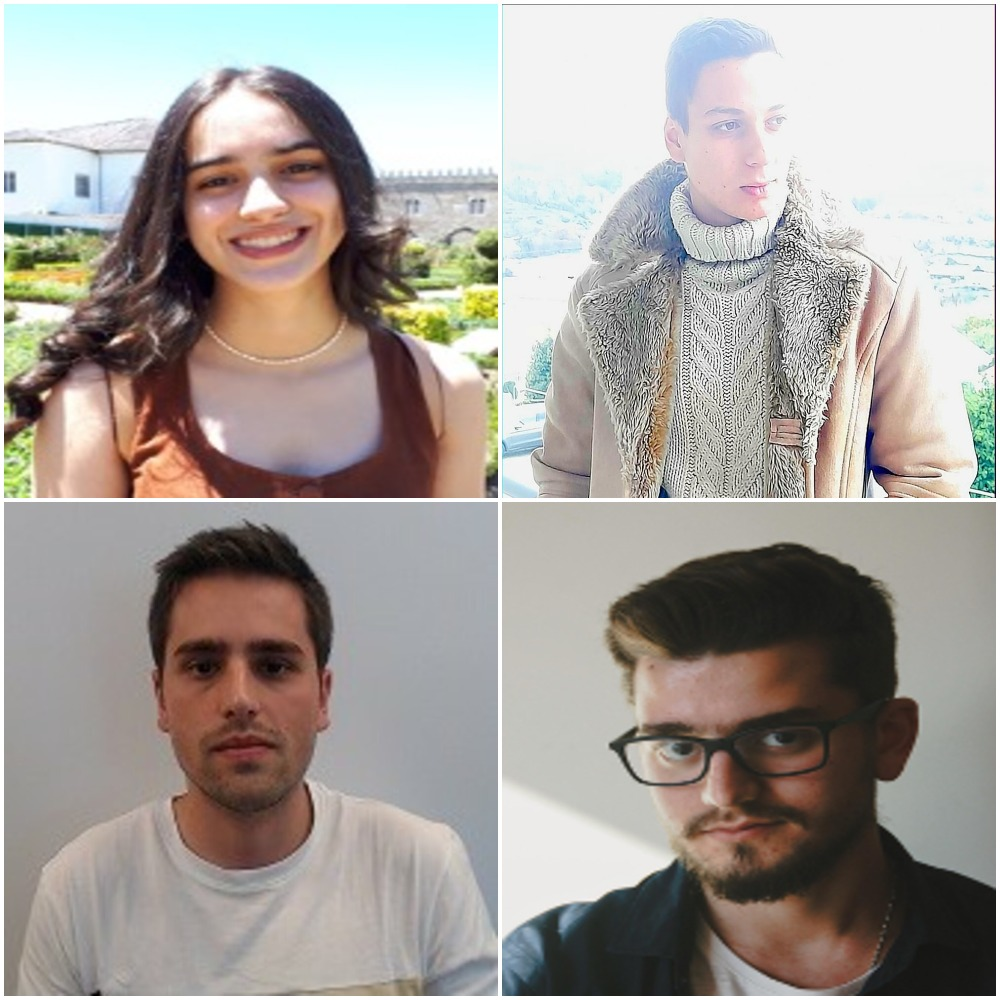
\includegraphics[width=0.7\linewidth]{us.jpg}
\end{center}
  \end{minipage}

\begin{abstract}  % resumo do documento
Neste relatório explicar-se-á a abordagem utilizada para construir a plataforma ComputationalMind, utilizando todos os conhecimentos práticos desenvolvidos ao longo do curso.
\end{abstract}

\tableofcontents % insere Indice

\chapter{Introdução}
\pagenumbering{arabic}

No âmbito da unidade curricular de Projeto da Licenciatura em Ciências da Computação, foi proposto o desenvolvimento de uma plataforma que permita inserir problemas/desafios para que os utilizadores possam, em modo jogo, responder a esses desafios. A plataforma deve ter uma interface de \emph{back-office} (BO) para armazenar os problemas/desafios (nomeadamente o seu enunciado, opções de resposta, resposta certa, faixa etária, etc). 
A interface de \emph{front-office} (FO) funciona em modo jogo para que os utilizadores possam responder aos desafios selecionados a partir do repositório criado no BO da plataforma. No modo jogo os utilizadores podem ter pontuações, prémios, ou outras formas de gamificação que os motivem e envolvam. \par
O presente relatório acompanha o processo de desenvolvimento do projeto.

\chapter{Enunciado do Projeto}

No âmbito do treino do Pensamento Computacional pretende-se criar uma plataforma que permita inserir problemas/desafios para que os utilizadores possam, em modo jogo, responder a esses desafios. A plataforma deve ter
uma interface de \emph{back-office} (BO) para armazenar os problemas/desafios (nomeadamente seu enunciado, opções de
resposta, resposta certa, faixa etária, etc). Um exemplo do tipo de exercícios que se pretende pode ser consultado na \emph{página\ da\ web} do bebras\footnote{http://bebras.dcc.fc.up.pt/problems/2021/problemas\_09\_10.pdf}.
A interface de \emph{front-office} (FO) funciona em modo jogo para que os utilizadores possam responder aos desafios
selecionados a partir do repositório criado no BO da plataforma. No modo jogo os utilizadores podem ter pontuações,
prémios, ou outras formas de gamificação que os motivem e envolvam.

\chapter{Concessão da Solução}

Para a elaboração de todo o projeto foi necessário recorrer a diversos recursos que ajudassem na realização do mesmo.

Antes de mais, o principal recurso utilizado foi a própria equipa de docentes que foi responsável por esclarecer e ajudar na tomada de decisões ao longo de todas as fases do projeto.

Inicialmente, com a escolha do tema foi necessário recolher uma série de artigos e questões com o intuito de nos familiarizar com os diferentes tipos de mídia que a plataforma teria de suportar e possibilitar a sua mesclação. 

Após essa pesquisa, surgiu a necessidade de ser feita modelação da Base de Dados, junto com a esquemização da página através da criação de Mockups \footnote{https://www.figma.com}. Na nossa visão estes passos representam um pouco os pilares e ideias sobre os quais o nosso projeto acenta, daí terem tomado uma parte significativa do nosso tempo.

De seguida, foram selecionadas as \emph{frameworks} para criação tanto da \emph{parte de suporte} como da \emph{interface frontal}, sendo elas o \emph{Django} \footnote{https://www.djangoproject.com} e o \emph{Reactjs} \footnote{https://reactjs.org}, assim como o \emph{TailWindCSS} \footnote{https://tailwindcss.com}. Nesta fase damos uma posição de destaque à fase de teste e adptação com as ferramentas, que levaram a uma etapa de muitas correções dos eventuais erros e de ajustes por forma a que nos certificarmos que o produto final correspondia às nossas expetativas, e às do público-alvo.

\chapter{Mockups}

Durante o processo de criação do site foi-nos proposto a criação de uma maquete (\emph{mockup}), que serviria como uma espécie de rascunho visual da forma como a \emph{página\ da\ web} poderia ser apresentada, permitindo-nos testar como os vários elementos visuais funcionam em conjunto.

Como o \emph{mockup} é um design estático, este não tem as funcionalidades oferecidas por um site vivo, por exemplo, não abrirá um \emph{pop-up} quando se clica no botão \emph{Login}, entre outros elementos. Fizemo-lo com o intuito de apresentar muitos dos elementos finais, da maneira como queríamos o \emph{design}, mas como em todas as maquetes algumas ideias foram modificas e eliminadas, devido a sugestões propostas pelos docentes da UC e para facilitar o processo de implementação.

Em última análise, percebemos que o \emph{mockup} de uma página deve ser criado para um propósito específico em mente. Que ofereceu à equipa a chance de ver como o objetivo podia ser alcançado, para que pudesse ser trazido à vida por meio da utilização de padrões de marca e criatividade visual. Sendo que aparece no ponto médio do processo de \emph{web\ design}.

\begin{figure}
     \centering
     \begin{subfigure}[b]{0.4\textwidth}
         \centering
         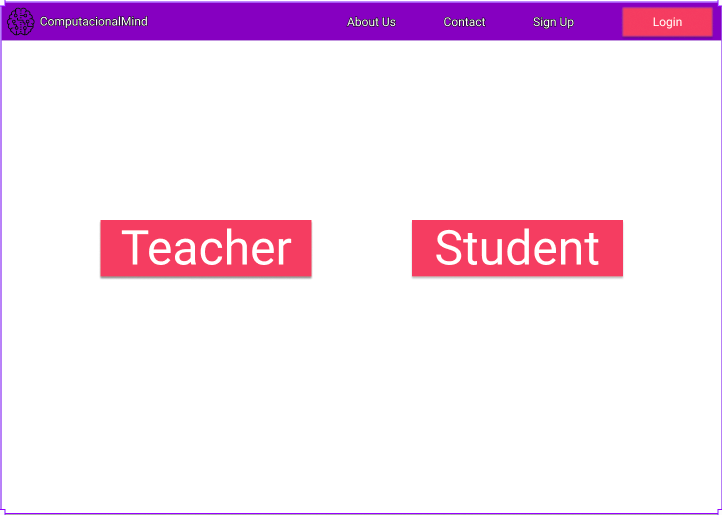
\includegraphics[width=\textwidth]{MockHome.png}
         \caption{Página Principal}
         \label{fig:MockHome}
     \end{subfigure}
     \hfill
     \begin{subfigure}[b]{0.4\textwidth}
         \centering
         \includegraphics[width=\textwidth]{MockLogin.png}
         \caption{Página de Login}
         \label{fig:MockLogin}
     \end{subfigure}
\end{figure}

\begin{figure}
     \centering
     %\begin{subfigure}[h!]{0.4\linewidth} Outra forma
     \begin{subfigure}[b]{0.4\textwidth}
         \centering
         %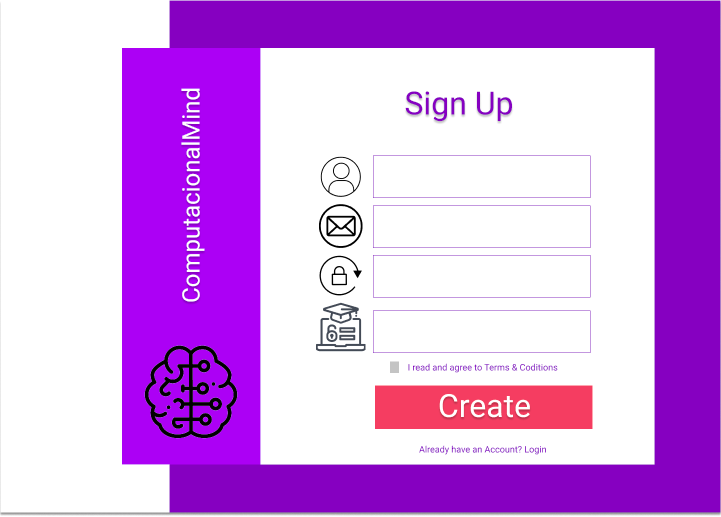
\includegraphics[width=\linewidth]{MockSingUp.png} Outra forma
         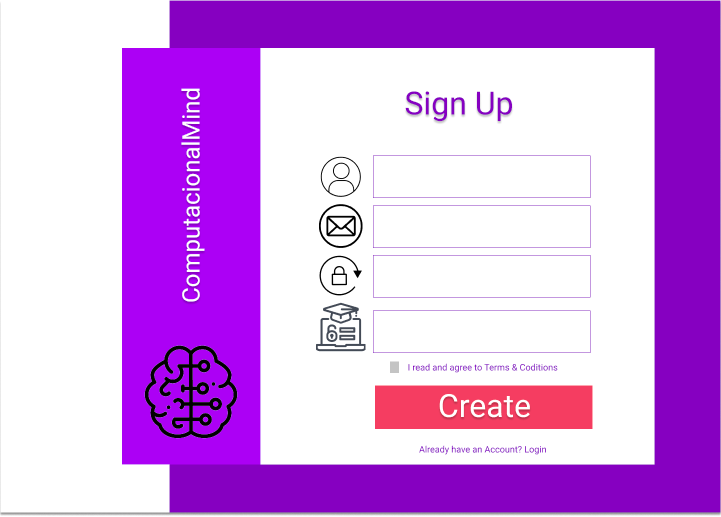
\includegraphics[width=\textwidth]{MockSingUp.png}
         \caption{Página de Criação de Conta}
         \label{fig:MockSingUp}
     \end{subfigure}
     \hfill
     \begin{subfigure}[b]{0.4\textwidth}
         \centering
         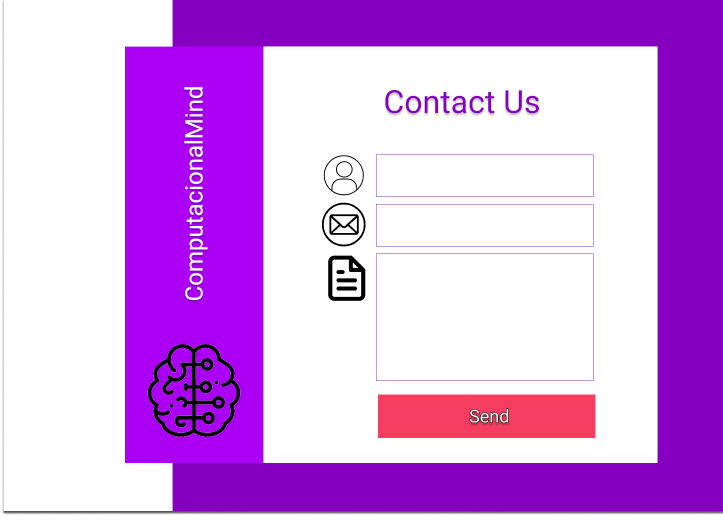
\includegraphics[width=\textwidth]{MockContactUs.png}
         \caption{Página de Contacto}
         \label{fig:MockContactUs}
     \end{subfigure}
     \hfill
     \begin{subfigure}[b]{0.4\textwidth}
         \centering
         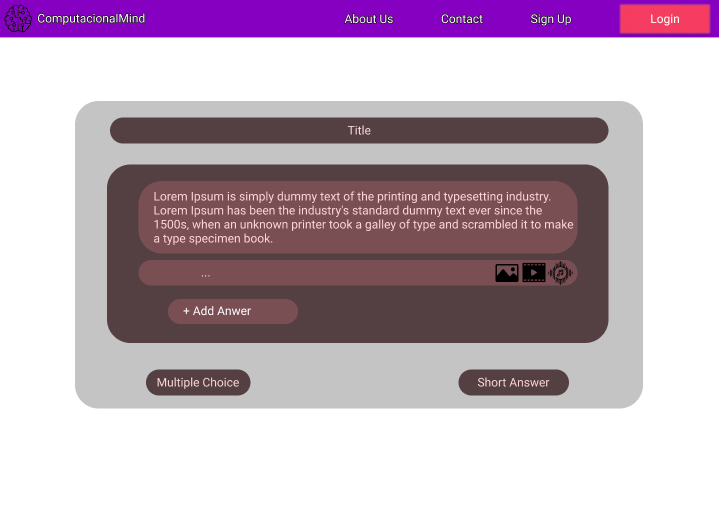
\includegraphics[width=\textwidth]{MockTeacherMenu.png}
         \caption{Menu de Inserção de Jogo}
         \label{fig:MockTeacherMenu}
     \end{subfigure}
     \hfill
     \begin{subfigure}[b]{0.4\textwidth}
         \centering
         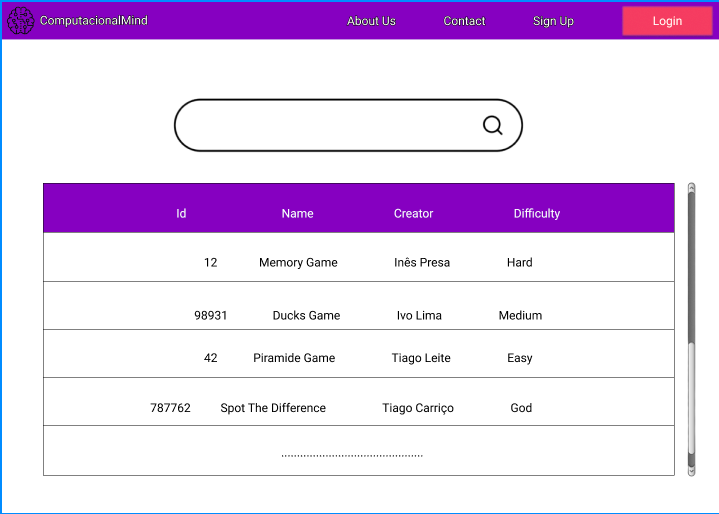
\includegraphics[width=\textwidth]{MockUserSelectGame.png}
         \caption{Menu de Seleção de Jogo}
         \label{fig:MockUserSelectGame}
     \end{subfigure}
     \hfill
     \begin{subfigure}[b]{0.4\textwidth}
         \centering
         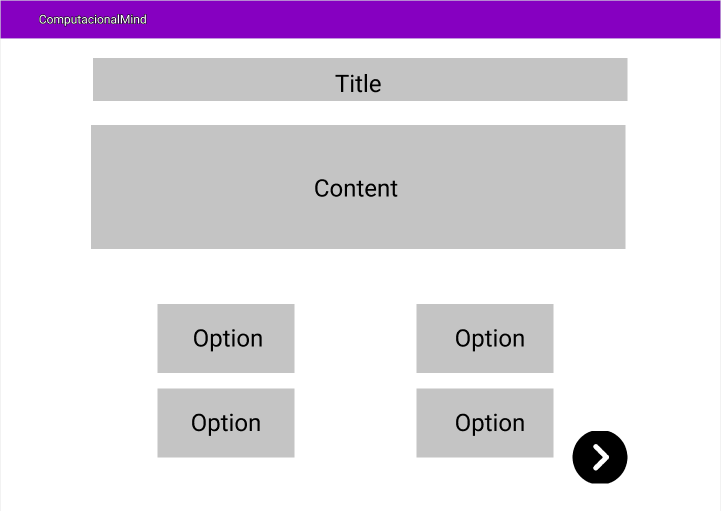
\includegraphics[width=\textwidth]{MockUserGameMC.png}
         \caption{Jogo de Escolha Múltipla}
         \label{fig:MockUserGameMC}
     \end{subfigure}
     \hfill
     \begin{subfigure}[b]{0.4\textwidth}
         \centering
         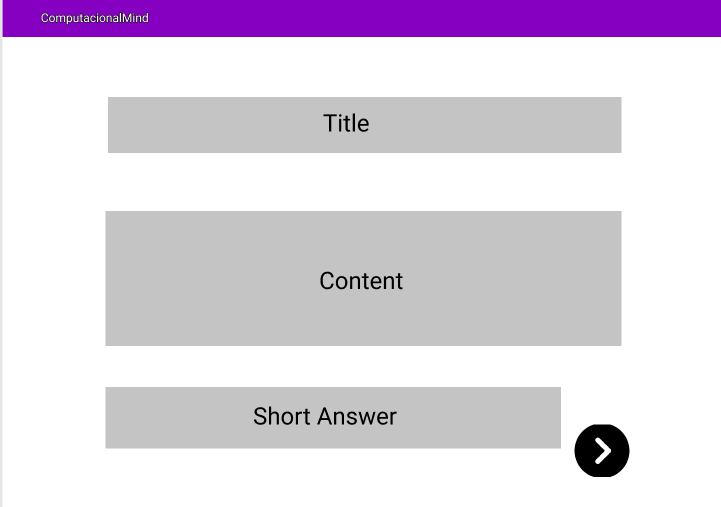
\includegraphics[width=\textwidth]{MockUserGameSA.png}
         \caption{Jogo de Resposta Curta}
         \label{fig:MockUserGameSA}
     \end{subfigure}
        %\caption{Mockups Realizados}
        %\label{fig:Mockups}
\end{figure}

\begin{figure}
    \begin{subfigure}[h!]{0.5\linewidth}
        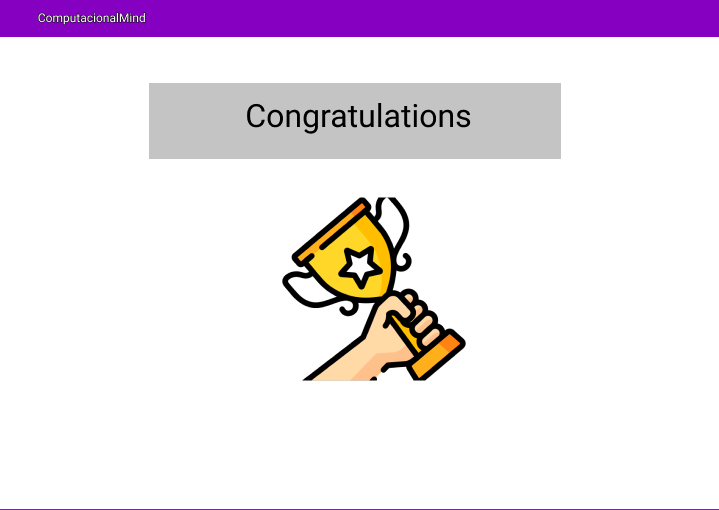
\includegraphics[width=\linewidth]{MockUserCongratulations.png}
        \caption{Resposta certa}
        \label{fig:MockUserCongratulations}
    \end{subfigure}
    \begin{subfigure}[h!]{0.5\linewidth}
        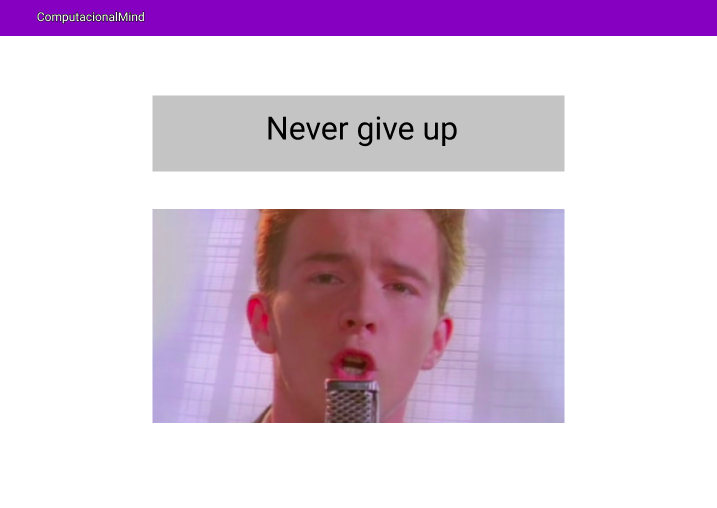
\includegraphics[width=\linewidth]{MockUserTryAgain.png}
        \caption{Resposta errada}
        \label{fig:MockUserTryAgain}
    \end{subfigure}
        %\caption{Design dos Mockups}
        %\label{fig:Mockups}
\end{figure}

\chapter{Base de Dados}

Para este projeto decidimos implementar uma Base de Dados Relacional que permita analisar e relacionar os dados do \emph{Computational Mind} com vista a melhor o serviço, uma vez que esta deverá possibilitar a manipulação e consulta dos dados de uma forma ágil e segura. 
Este será um processo trabalhoso, mas que trará grandes frutos no futuro, uma vez que será substancialmente mais eficiente, especialmente na atualização, consulta e tratamento dos dados, o que permitirá alcançar todos os objetivos propostos pela equipa docente. Para além disso, será também um sistema mais fiável, visto que garantirá uma uniformização dos dados, garantindo que qualquer interveniente que pretenda consultar ou alterar os dados o fará de uma forma mais segura e controlada.

\section{Identificação e caracterização das entidades}

\subsection{Author}
Um autor é identificado por um \textbf{código}, devendo ter também uma referência do seu \textbf{nome}, \textbf{\emph{e-mail}} e \textbf{\emph{password}}.

\subsection{Player}
Um jogador é identificado por um \textbf{código}, devendo ter também uma referência do seu \textbf{nome}, \textbf{data de aniversário}, \textbf{\emph{e-mail}} e \textbf{\emph{password}}

\subsection{Question}
Uma questão é identificado por um \textbf{código},devendo ter também uma referência ao \textbf{autor}, um um \textbf{título}, um identificador do \textbf{tipo} (resposta curta, escolha múltipla ou verdadeiro e falso), uma \textbf{classificação}, a \textbf{dificuldade} e a \textbf{idade mínima}.

\subsection{Content}
Um conteúdo é identificado por uma referência à \textbf{questão}, uma \textbf{ordem} pela qual as questões aparecem, o \textbf{tipo} do conteúdo e os \textbf{links/imagens/vídeos} associados. 

\subsection{Option}
Uma opção é identificado por um \textbf{código}, uma referência à \textbf{questão}, a \textbf{resposta} para serem feitas as verificações e a \textbf{opção correta}.

\subsection{History}
Um histórico é identificado por \textbf{código}, uma referência ao \textbf{jogador}, uma referência à \textbf{questão}, a \textbf{data} que o jogador respondeu à questão, as suas \textbf{respostas} e quais \textbf{acertou}.

\section{Identificação e caracterização dos relacionamentos}

\begin{center}
\begin{tabular}{ |c|c|c|c|c| } 
 \hline
 \bf{Entidade} & \bf{Multiplicidade} & \bf{Relacionamento} & \bf{Multiplicidade} & \bf{Entidade} \\ 
 \hline
 Question & 1..N & tem & 1 & Author \\ 
 \hline
 Option & 1..N & tem & 1 & Question \\ 
 \hline
 History & 1..N & tem & 1 & Question \\ 
 \hline
 History & 1..N & tem & 1 & Player \\ 
 \hline
 Content & 1..N & tem & 1 & Question \\ 
 \hline
\end{tabular}
\end{center}

\section{Modelo Lógico}

\begin{figure}[H]
\centering
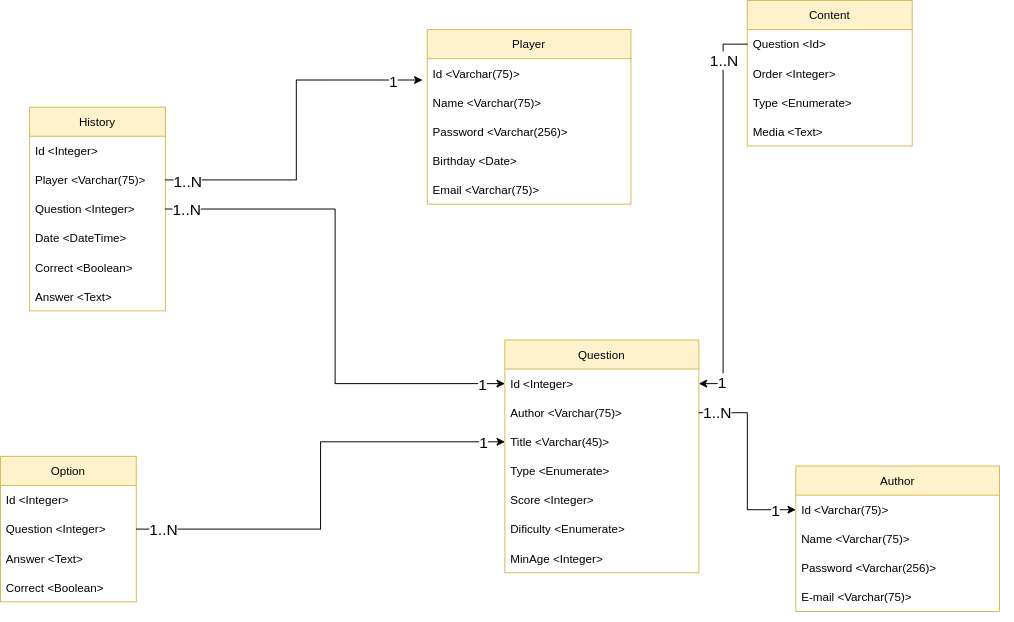
\includegraphics[width = 14cm,height = 10cm]{EsqLog.png}
\caption{Esquema Lógico}
\label{fig:EsqLog}
\end{figure}

\chapter{Back-end}

\section{Ferramentas}

Para o desenvolvimento da  \emph{parte secundária} utilizou-se \emph{Django} e \emph{Django REST Framework}.

\section{Django}

\emph{Django} é uma \emph{framework} gratuito e de código aberto, com o intuito de facilitar e acelerar o desenvolvimento \emph{web}, escrito em Python, que utiliza o padrão \emph{model-template-view} (MTV) e o princípio \emph{don't repeat yourself} (DRY) através do aproveitamento máximo de código já feito. O \emph{web\ server}, pode ajudar os desenvolvedores a produzir de forma eficiente um FO ou BO rico em recursos, seguro e escalável.

O \emph{Django REST Framework} é um conjunto de ferramentas utilizado para construir \emph{APIs} (Interfaces de Programação de Aplicações) para \emph{Web}.

Apesar do \emph{Django} permitir fazer tanto \emph{front-end} como \emph{back-end}, a utilização de uma \emph{REST API} permite desenvolver uma \emph{parte de suporte} mais genérico, e torna possível desenvolver uma \emph{parte frontal} para vários tipos de dispositivos no futuro. Ou seja, assim a aplicação torna-se mais escalável. 

\section{Objetivo}

O \emph{back-end} do projeto tem como objetivo fazer a ligação entre a Base de Dados e a \emph{interface frontal}, tendo sido desenvolvido ainda uma \emph{REST API} que será "consumida" pela mesma.
\newpage
\section{Desenvolvimento}

No processo de desenvolvimento utilizou-se a base de dados previamente implementada no \emph{MySQL Workbench} para se fazer a construção dessas mesmas entidades e relacionamentos no \emph{Django} com o intuito de possibilitar a comunicação entre ambos foi necessário alterações o esquema mais concretamente a eliminação das chaves primárias compostas.

A comunicação entre o \emph{Django} e a \emph{parte frontal} através da \emph{REST API} é feita com o uso de ficheiros em formato \emph{JSON}. Para tal, o \emph{Django} possui funções especificas para serializar e desserializar os dados. O uso dá-se da seguinte forma, o \emph{front-end} faz uma pedido através da \emph{REST API}, de seguida este pedido é analisado pelo \emph{Django} e caso esteja correto os dados requeridos são copiados da base de dados, serializados e enviados em formato \emph{JSON} para a \emph{interface frontal}. A comunicação inversa também é possível mas os dados são desserializados e estando corretos, serão inseridos na base de dados.

\begin{figure}[h]
\centering
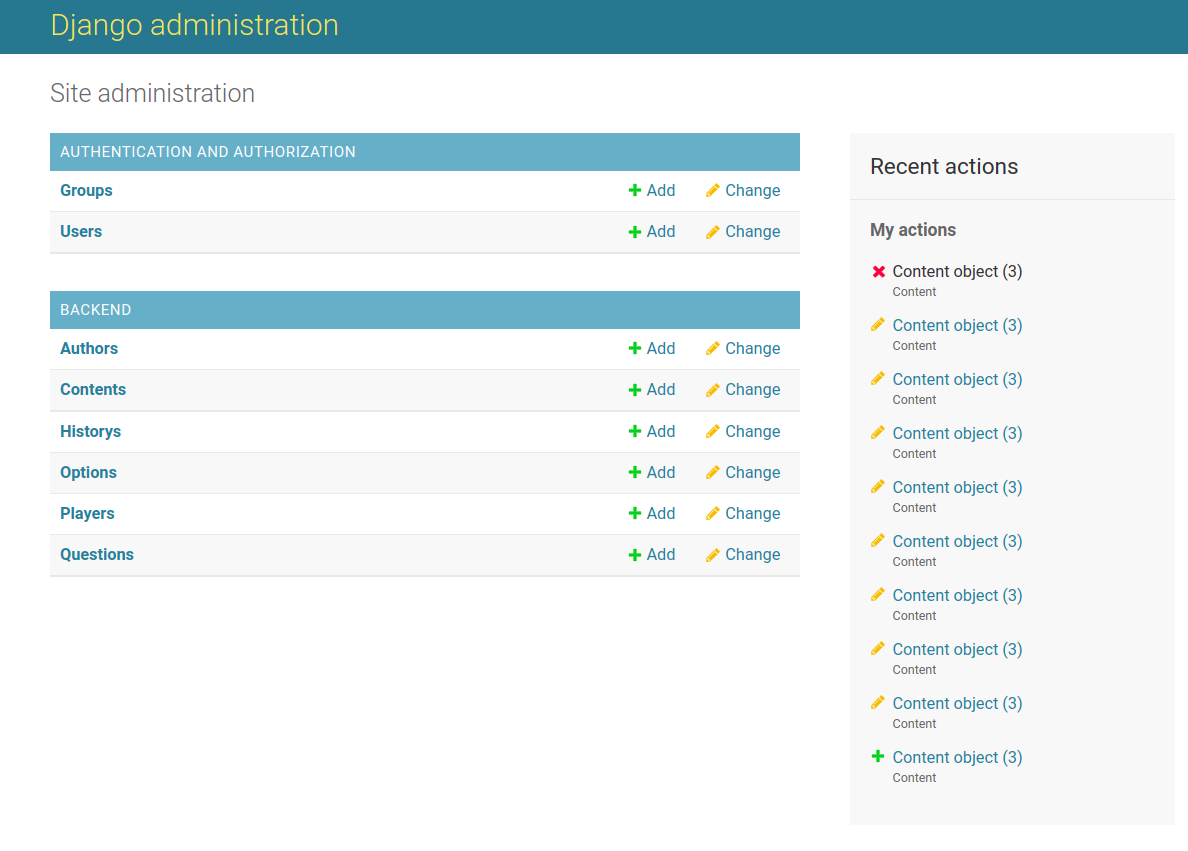
\includegraphics[width = 14cm,height = 10cm]{apiDjango.png}
\caption{REST API}
\label{fig:pagDJang}
\end{figure}

\chapter{Front-End}

\section{Ferramentas}
Para o desenvolvimento do  \emph{front-end} utilizou-se \emph{React} e \emph{TailWindCSS}.

\section{React e TailWindCSS}

\emph{React.js} é uma biblioteca \emph{JavaScript} de código aberto usada para construir o \emph{front-end} para aplicativos e páginas \emph{web} de página única. Sendo usado para lidar com a camada de visualização para os aplicativos da \emph{Web} e móveis. O \emph{React} também nos permite criar componentes de interface do usuário reutilizáveis para que os desenvolvedores criem grandes aplicativos da \emph{Web} que possam alterar dados sem que seja necessário recarregar a página. O seu principal objetivo é ser rápido, escalável e simples. Este funciona apenas em interfaces de usuário no aplicativo, o que corresponde à exibição do modelo \emph{Model-View-Controller} (MVC), podendo ser usado em conjunto com outras bibliotecas ou \emph{frameworks\ JavaScript}, como \emph{Angular\ JS} em MVC.

\emph{Tailwind\ CSS} é basicamente um \emph{framework\ CSS} utilitário para construir de forma rápida interfaces de utilizador personalizadas, sendo uma estrutura \emph{CSS} altamente personalizável e de baixo nível que fornece todos os blocos de construção necessários para criar \emph{designs} sob medida, sem que seja necessária a escrita de \emph{CSS} como na abordagem tradicional.

\section{Objetivo}

O \emph{front-end} é responsável por possibilitar a interação do utilizador com a página dentro de uma aplicação \emph{web} e cobrindo as questões da política de privacidade.

\section{Desenvolvimento}

Cenas

\chapter{ComputationalMind}

Ao longo deste semestre desenvolvemos a página do \emph{ComputationalMind} até que o produto final fosse semelhante ao que foi idealizado e apresentado nos capítulos anteriores. Em seguida, será demonstrado o funcionamento e onde se podem encontrar todas as funcionalidades implementadas.

\section{Página inicial (Sem sessão iniciada)}

Na página inicial consideramos que o utilizador pode ser um \emph{Player} que apenas usufrui dos jogos disponibilizados na plataforma pelo \emph{Author} que é a entidade que criou o jogo.

\begin{figure}[h]
    \centering
    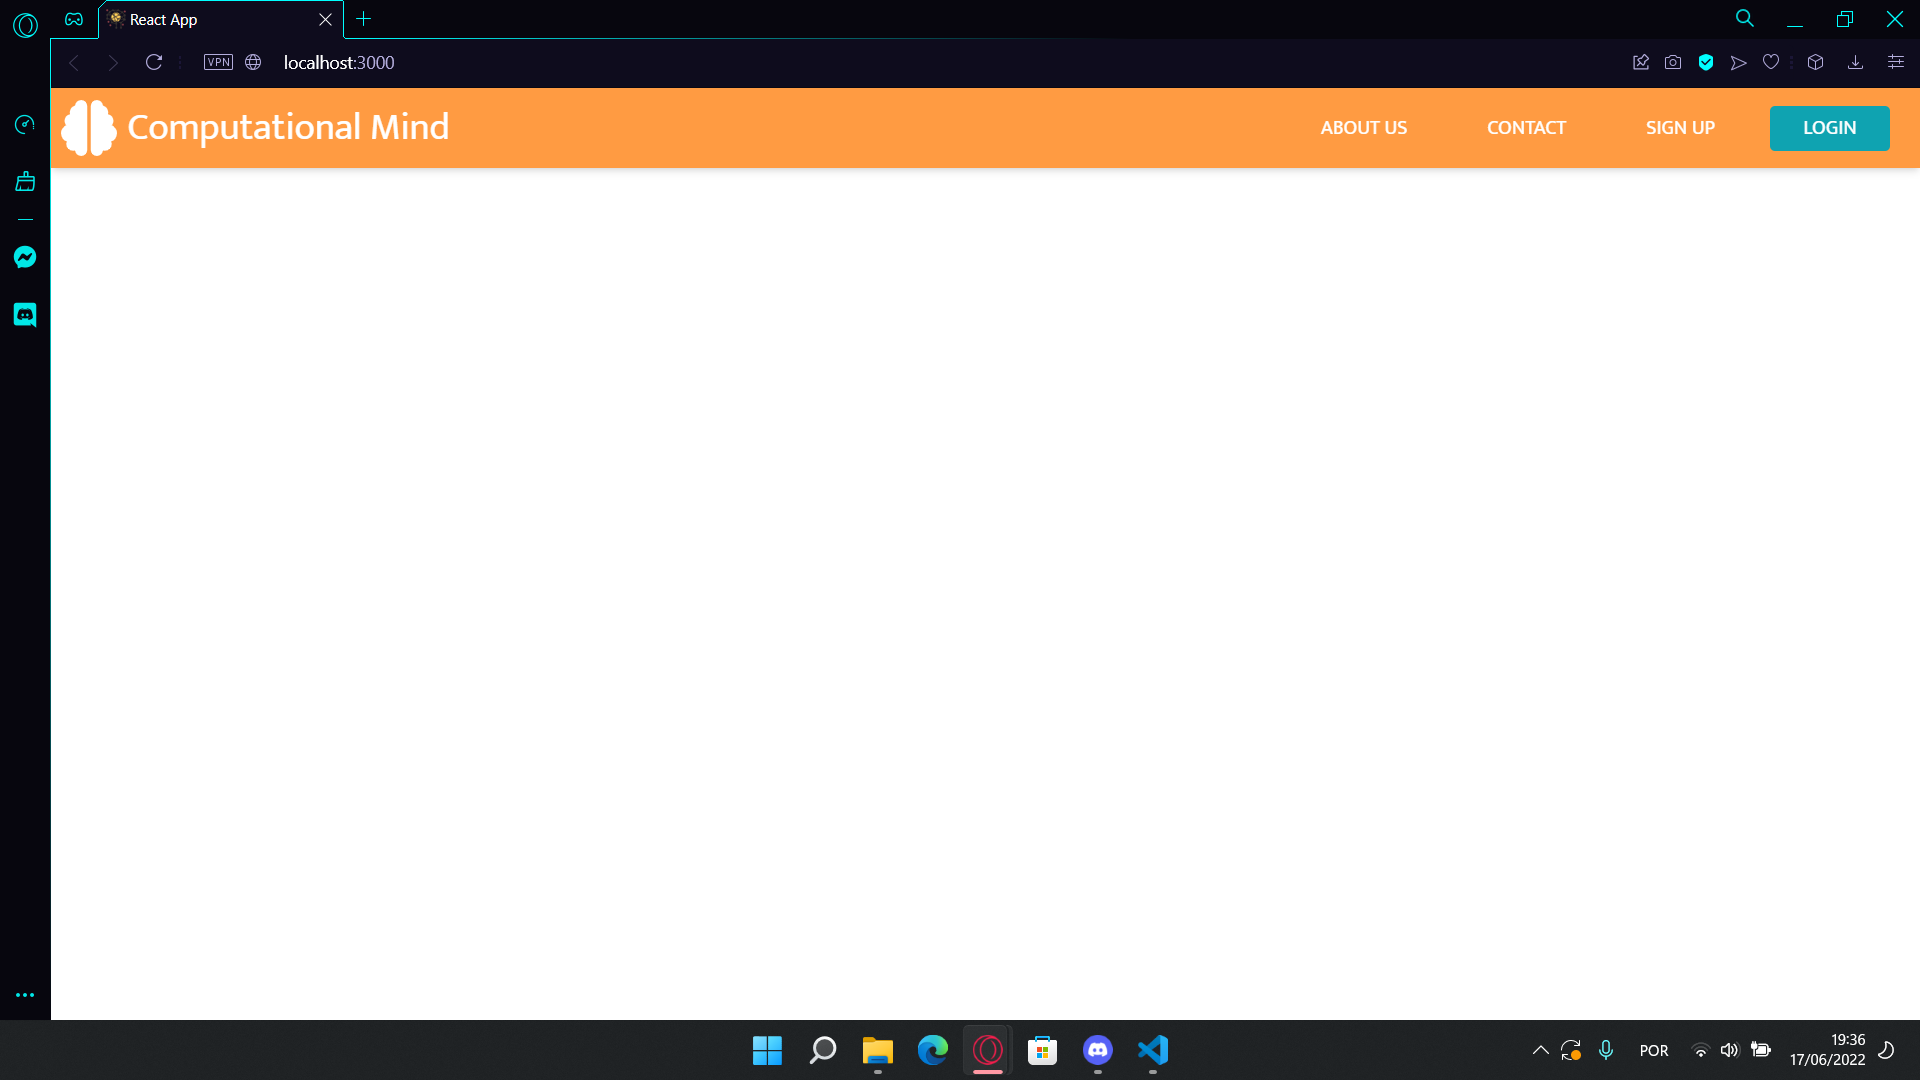
\includegraphics[width = 10cm]{pagIni.png}
    \caption{Página Principal}
    \label{fig:pagIni}
\end{figure}

\newpage

\section{About Us}

Nesta secção incorporamos informação sobre o propósito da página.

\begin{figure}[h]
    \centering
    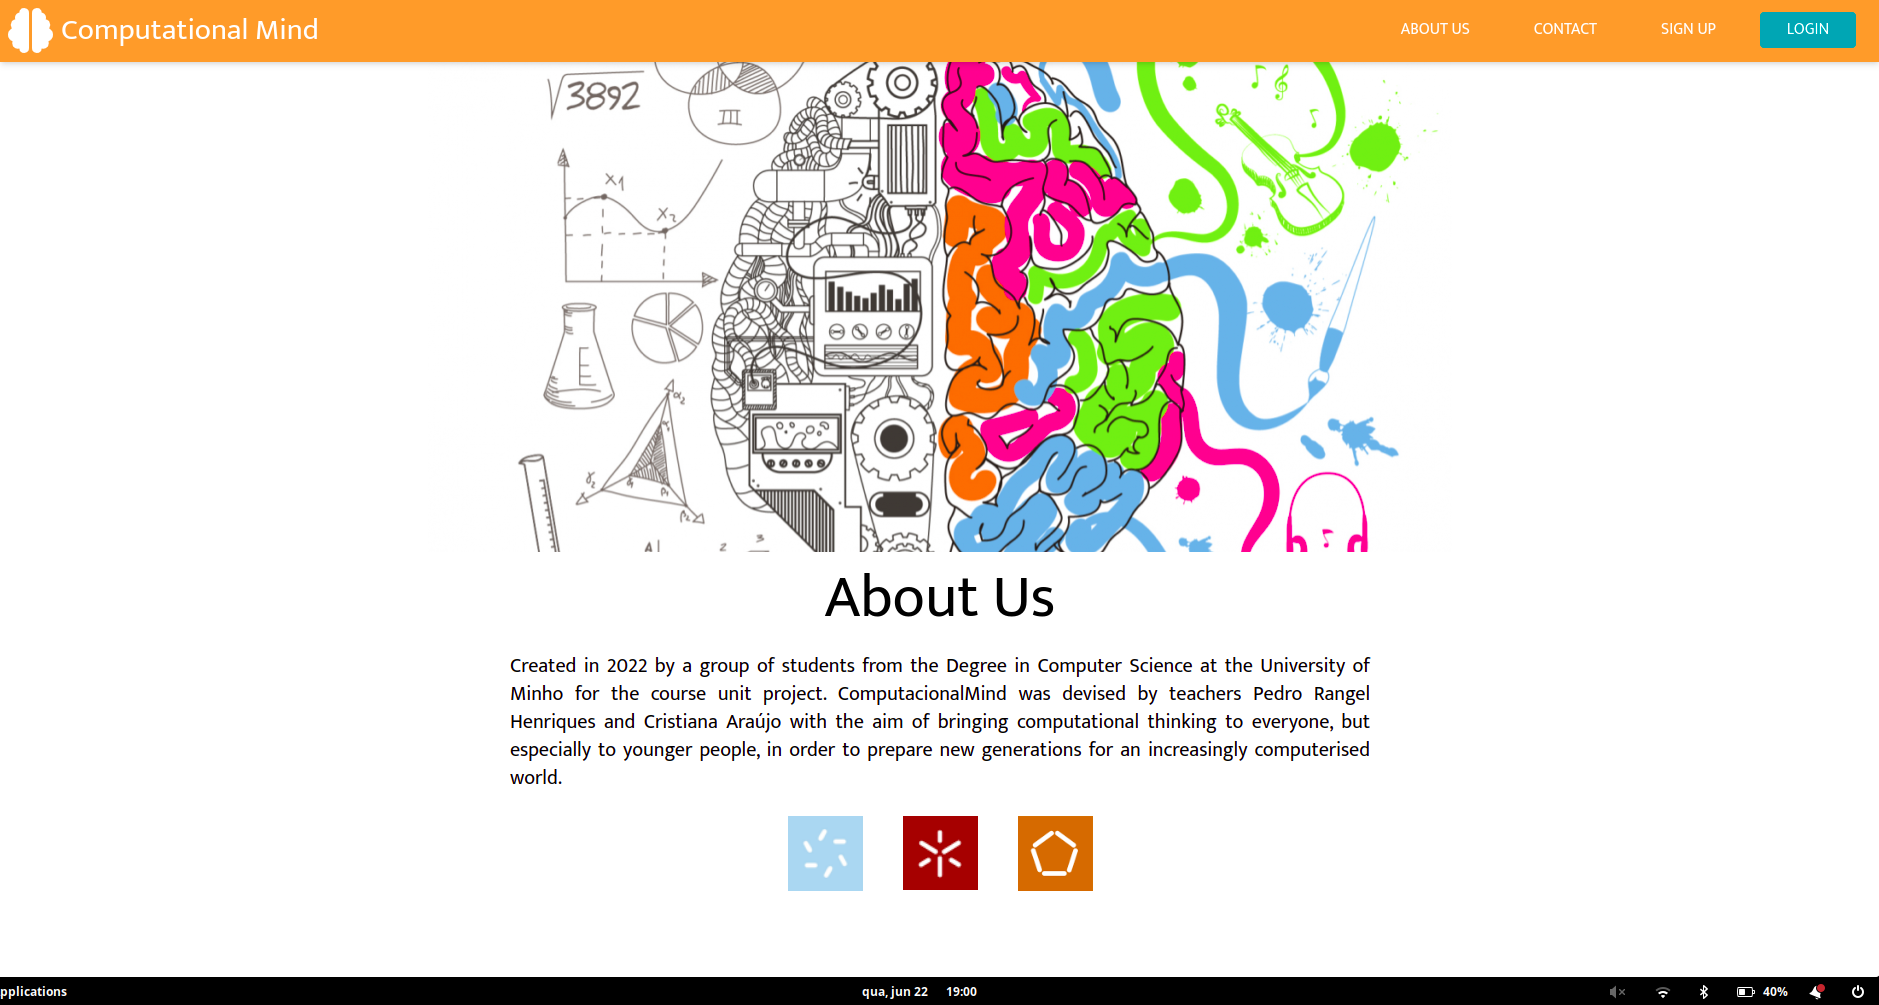
\includegraphics[width = 10cm]{aboutUs.png}
    \caption{About Us}
    \label{fig:abUs}
\end{figure}

\section{\emph{Login} / \emph{Sign Up}}
Após a escolha de uma das opções disponibilizadas na página inicial os utilizadores seram redirecionados para a página de \emph{Login} / \emph{Sign Up}. 

Nesta página é possível um utilizador autenticar-se ou efetuar o seu registo no site. 

A página de autentificação é igual para ambos os utilizadores, a única diferença na página de \emph{Sign Up} do \emph{Player Sign Up} para a do \emph{Author Sign Up} é que na do \emph{Player} é relevante saber a idade para serem apresentados jogos mais adequados à sua faixa etária enquanto que na do \emph{Author} essa informação não é relevante. 

\begin{figure}[h]%
    \centering
    \subfloat[\centering Página de \emph{Login}]{{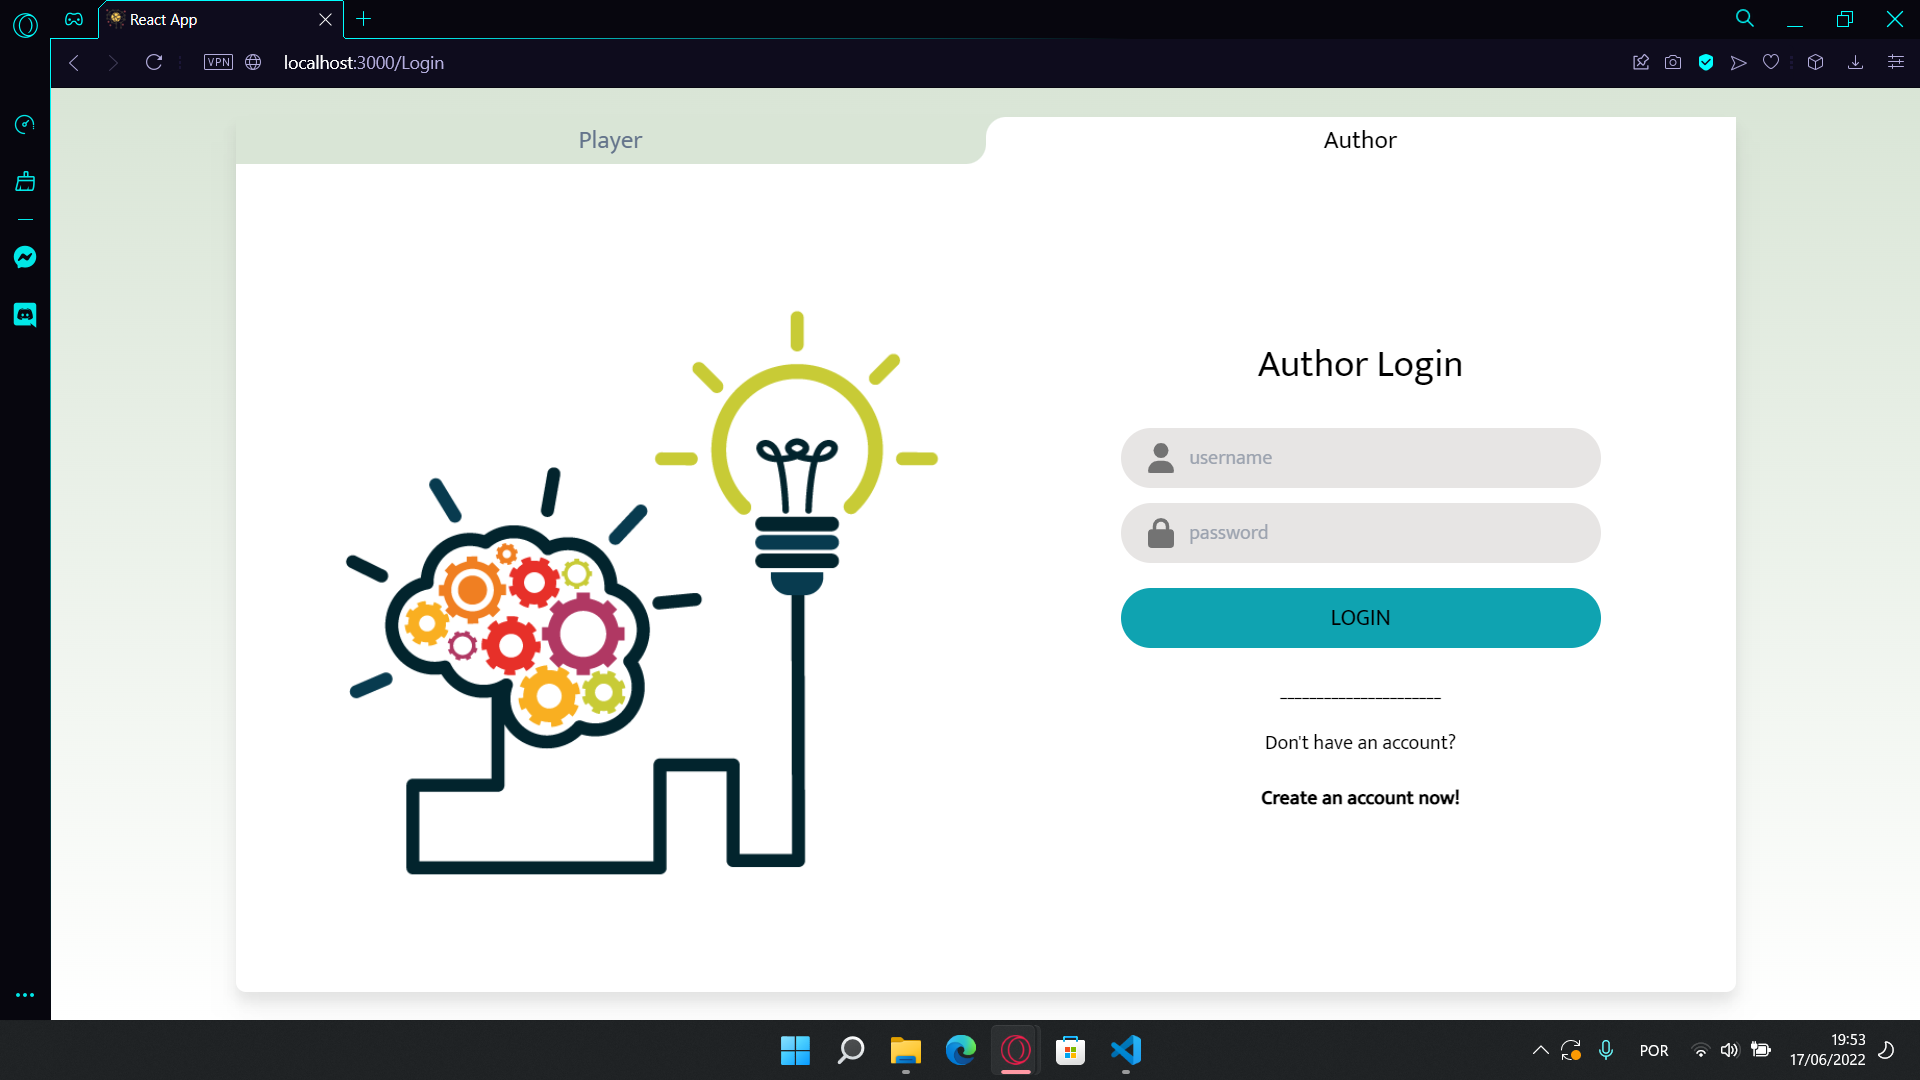
\includegraphics[width=5cm]{log.png} }}%
    \qquad
    \subfloat[\centering Página de \emph{Sign Up Author}]{{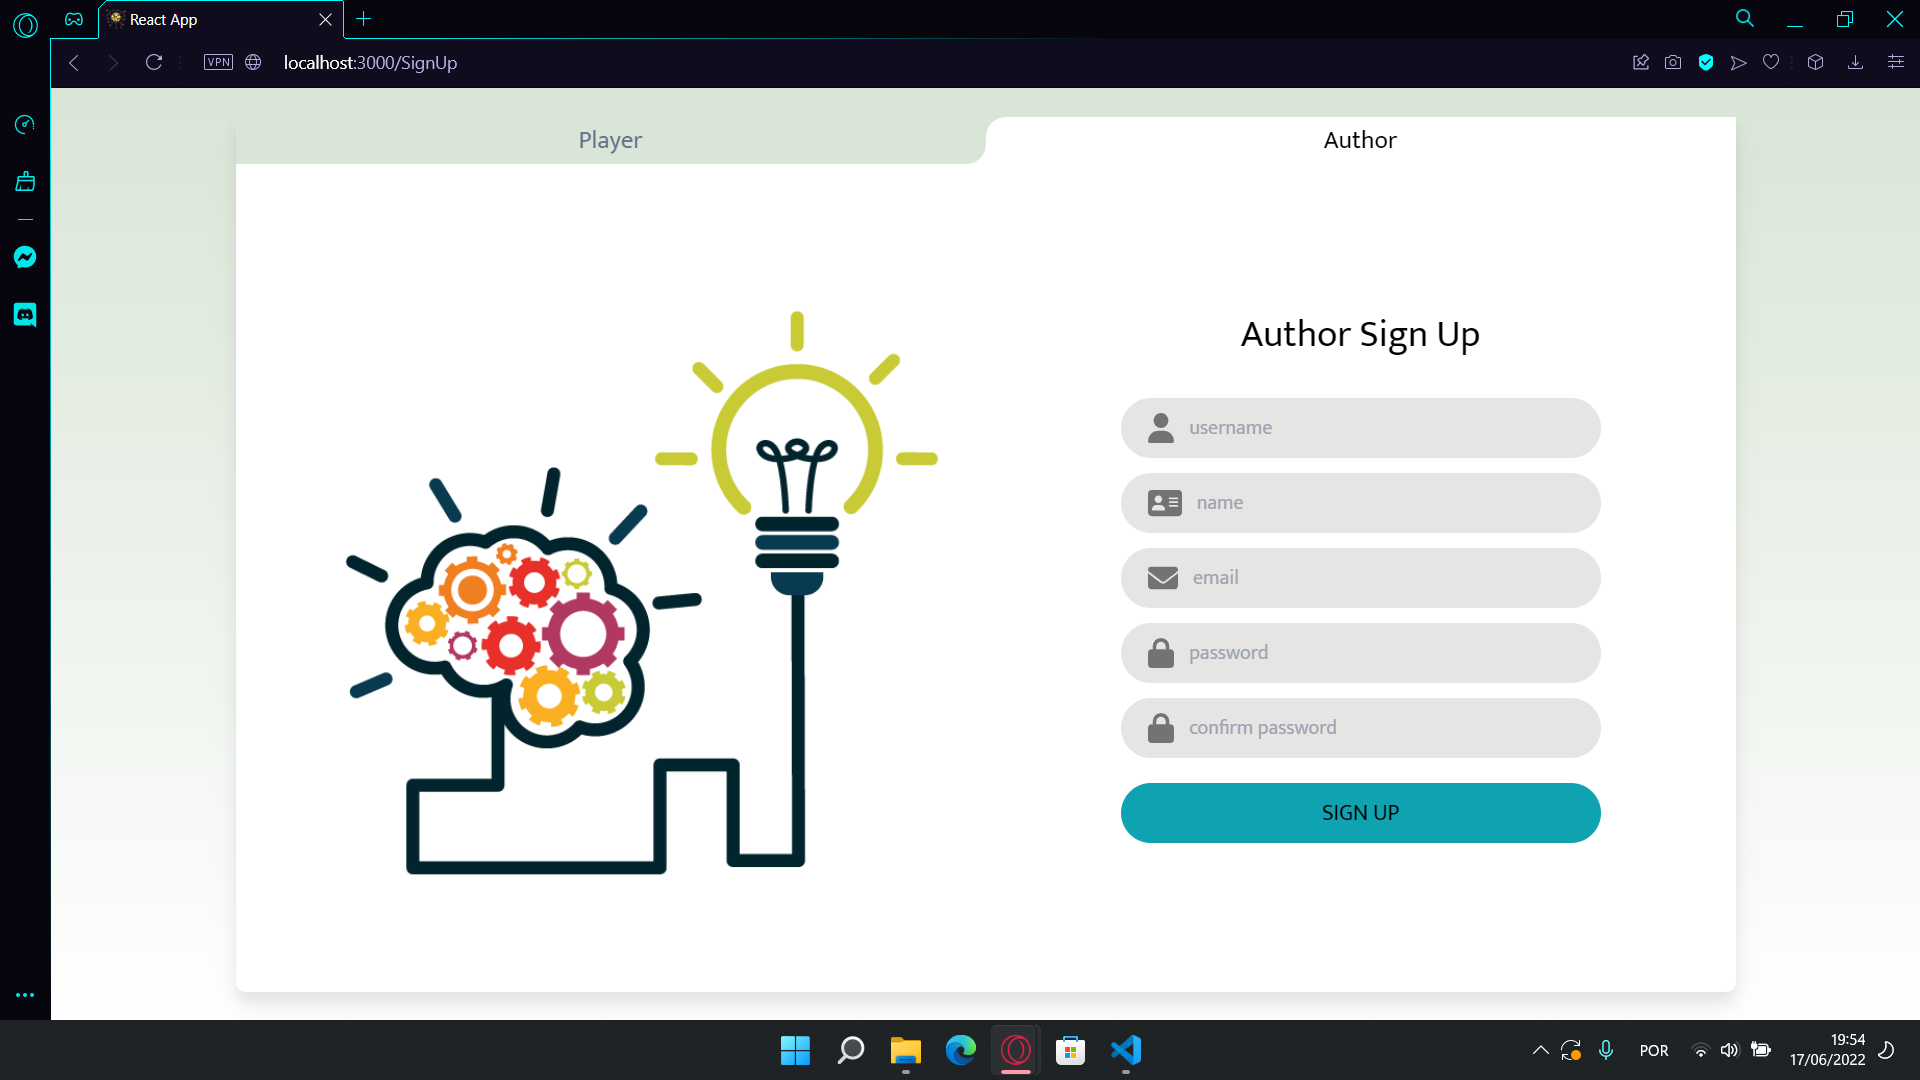
\includegraphics[width=5cm]{sigUpA.png} }}%
    \qquad
    \subfloat[\centering Página de \emph{Sign Up Player}]{{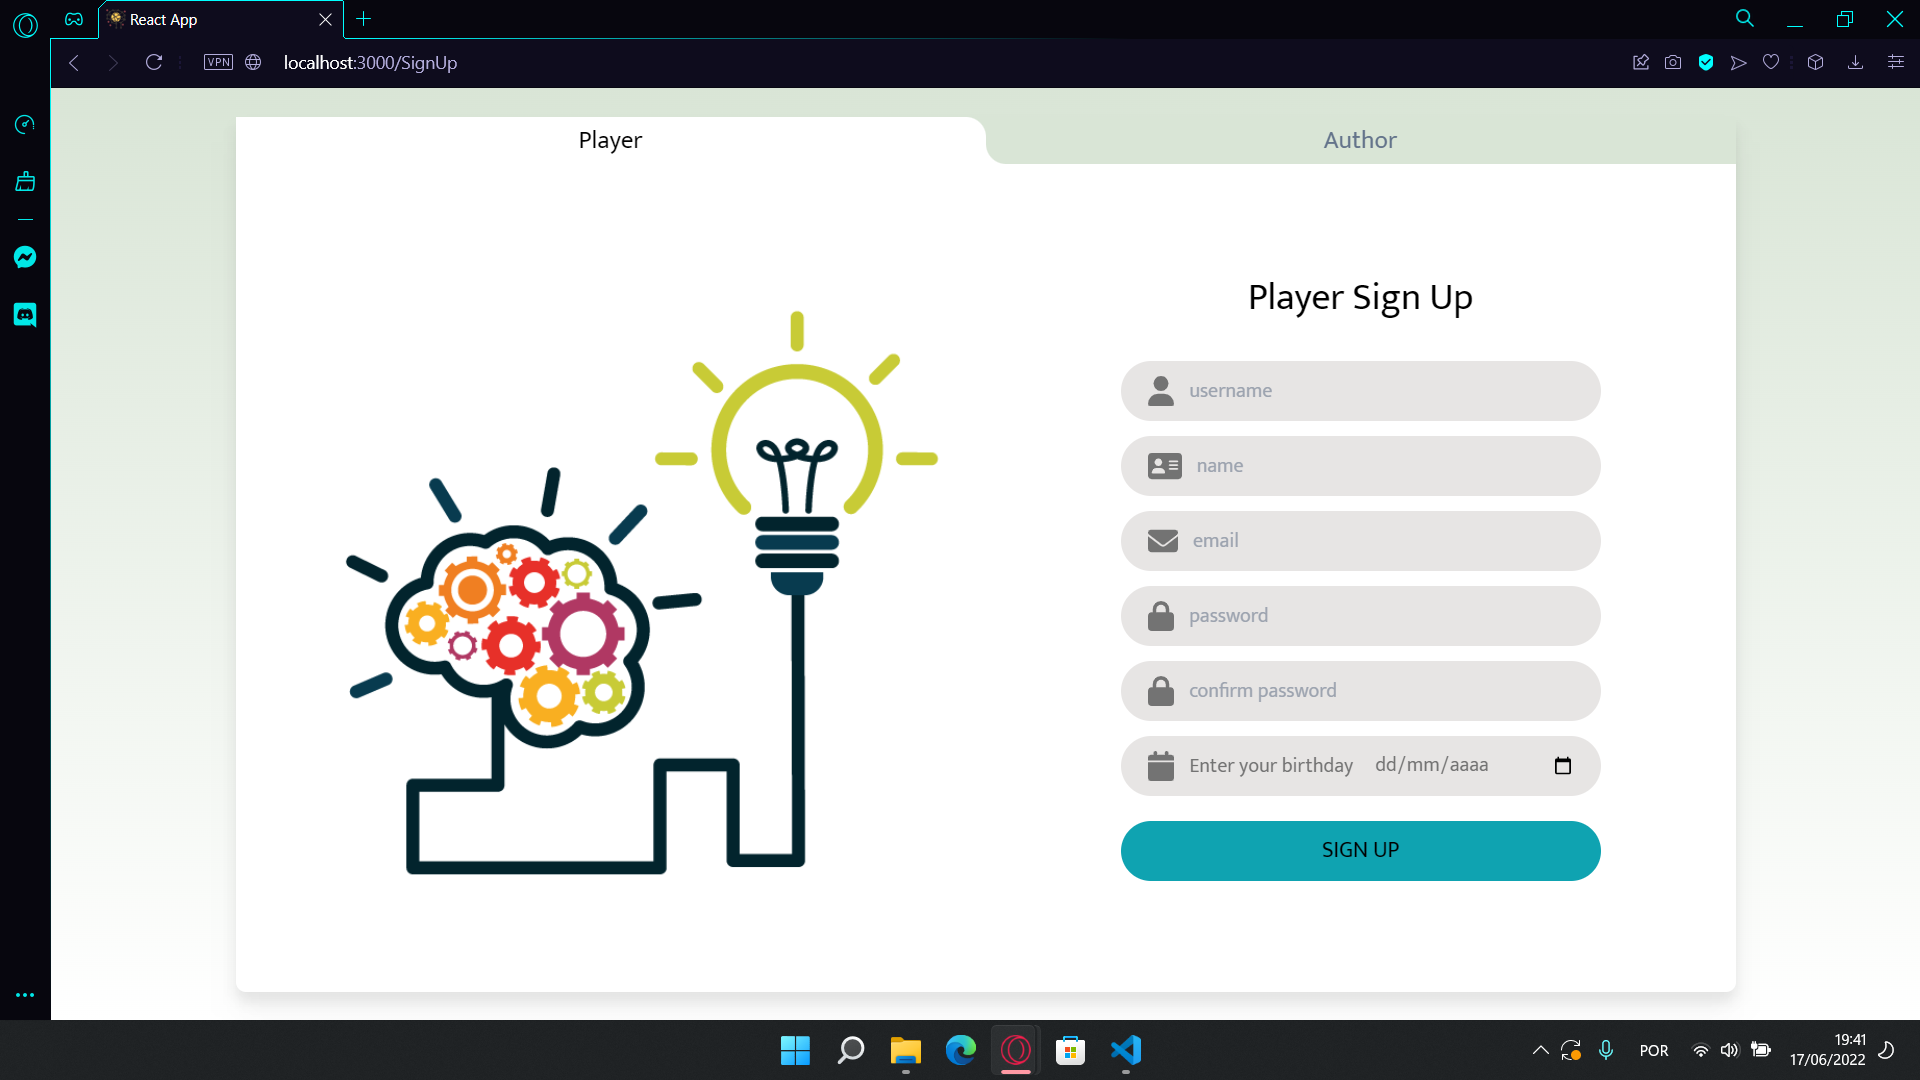
\includegraphics[width=5cm]{sigUpP.png} }}%
    \caption{Página de \emph{Login} e Registo}%
    \label{fig:log&sigUp}%
\end{figure}

\newpage

\section{Escolha de jogos para \emph{Player} ou \emph{Author}}
Em seguida, ambos os utilizadores são redirecionados para uma página onde se lista todos os jogos que estão disponíveis para jogar.

\begin{figure}[h]
    \centering
    \includegraphics[width = 10cm]{pagJog.png}
    \caption{Página de Jogos}
    \label{fig:pagJog}
\end{figure}

\section{Menu do \emph{Author}}
O \emph{Author} é um utilizador especial, diferindo de um utilizador normal pelo facto de existir uma secção chamada \emph{Creat New Game} onde poderá criar os diferentes tipos de jogos referido nos capítulos anteriores.

\begin{figure}[h]
    \centering
    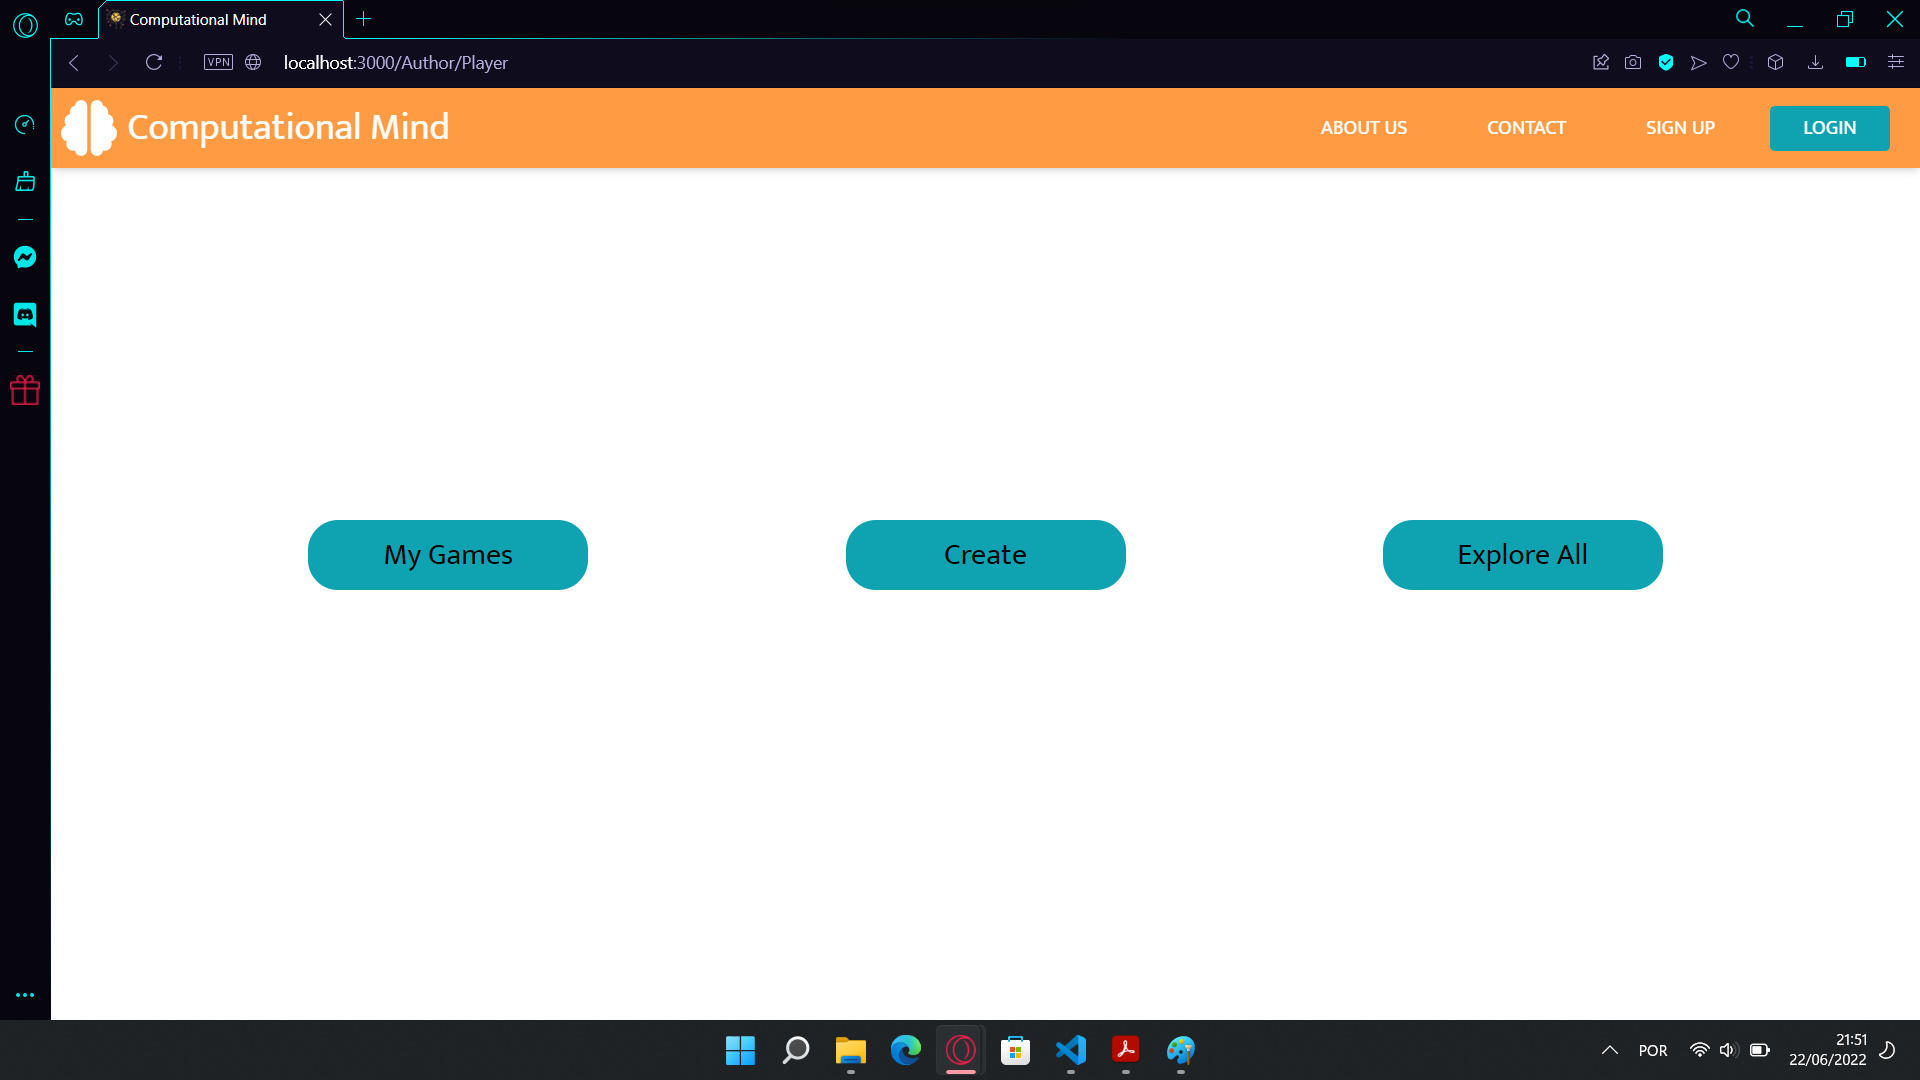
\includegraphics[width = 10cm]{menuAut.png}
    \caption{Menu do \emph{Author}}
    \label{fig:menuAut}
\end{figure}

\newpage

\section{Criação de novos Jogos}
Nesta nova aba oferecemos todas as ferramentas suportadas pela página para que o \emph{Author} consiga criar novo conteúdo para a mesma.
\begin{figure}[h]
    \centering
    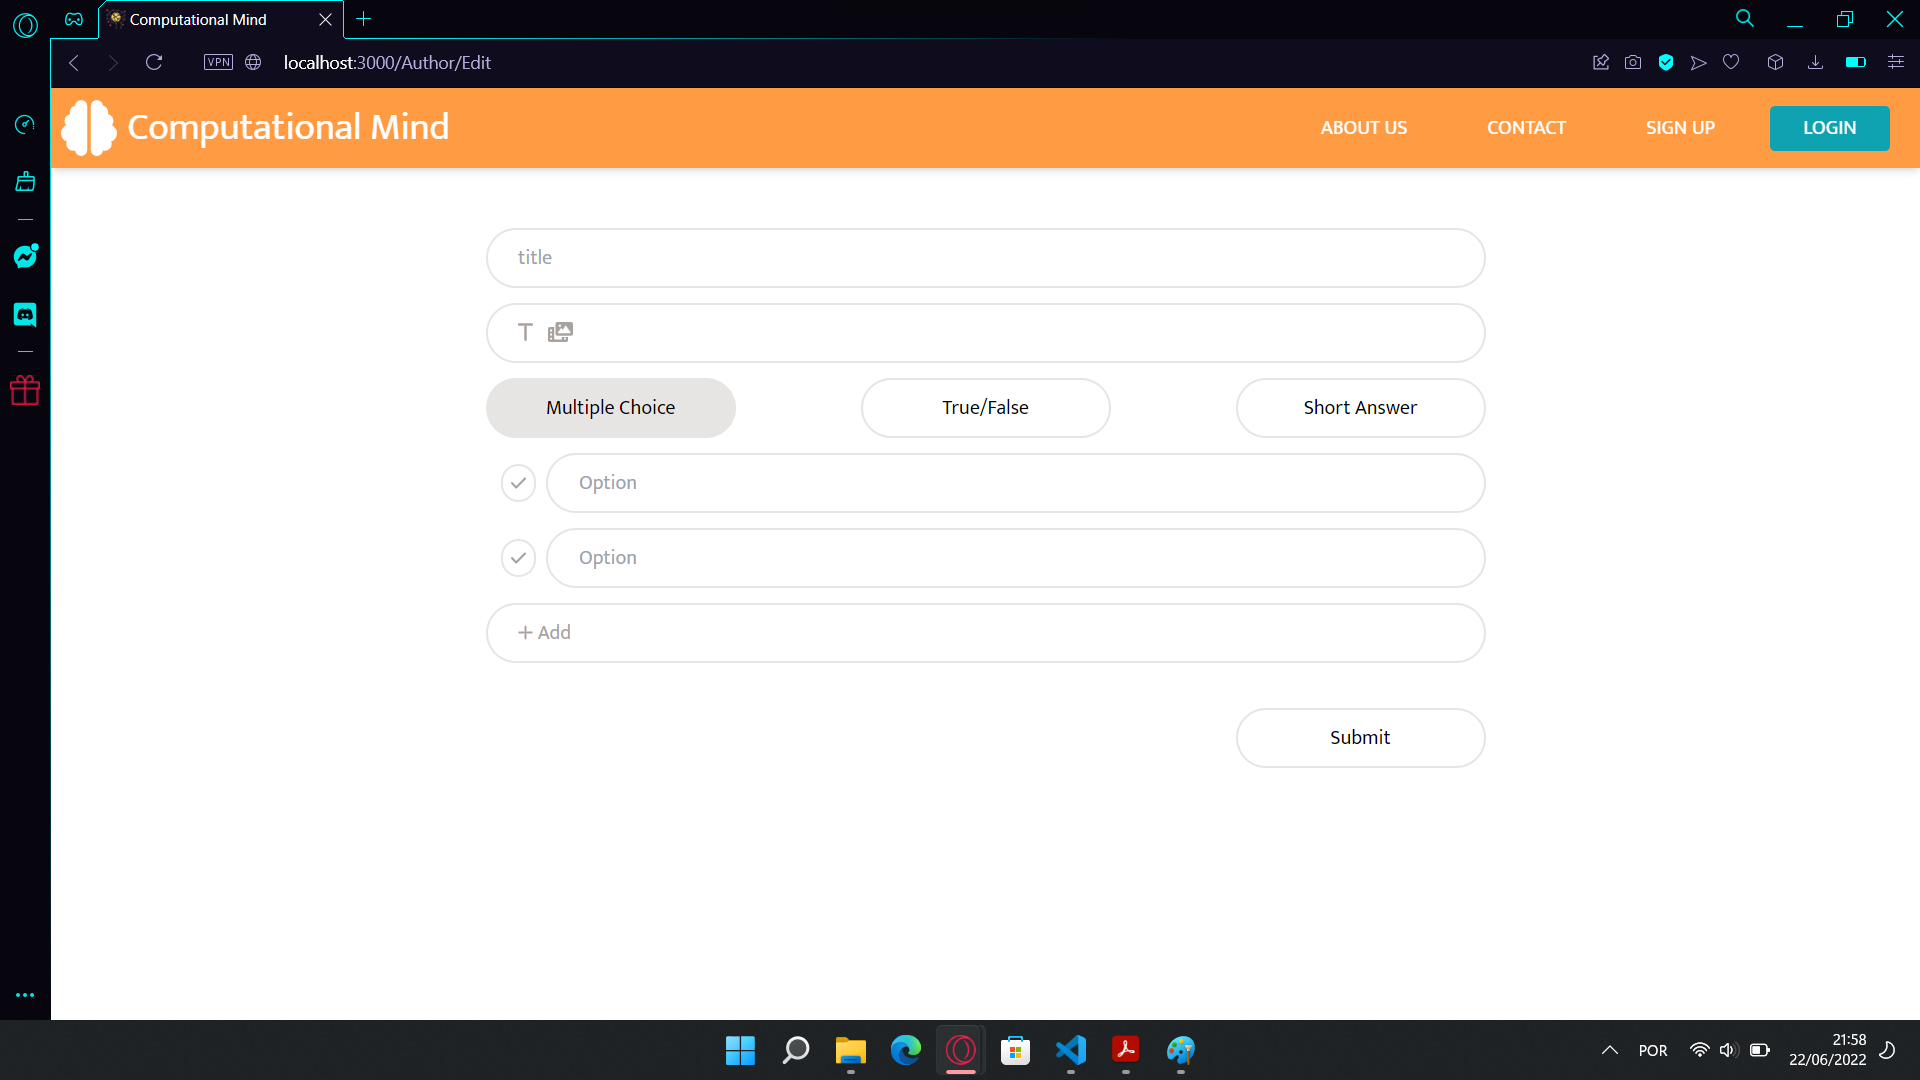
\includegraphics[width = 10cm]{editAut.png}
    \caption{Menu para Criação de Jogos pelo \emph{Author}}
    \label{fig:editAut}
\end{figure}

\section{Página inicial (Com sessão iniciada)}

Quando um utilizador se regista ou autenticação, é redirecionado para a página principal da aplicação. Aqui é possível ver todas as opções de países e categorias disponíveis, bem como selecioná-los de forma a filtrar as notícias. Além disto, consegue-se ver as trending news, e pode-se aceder a outras páginas da aplicação.

Demo da pagina, login, user, autor, apresentação das funcionalidades,...

\chapter{Conclusão}

Conclui-se desta forma a apresentação do Projeto para o ano letivo 2021/2022.

\section{Comentários}

Temos de realçar que o projeto não se encontra totalmente finalizado, na medida em que algumas das funcionalidades planeadas acabaram por não ser implementadas na versão final. Desta forma, o projeto final é apenas uma “amostra” daquele que foi inicialmente idealizado estando presentes apenas as funcionalidades consideradas mais importantes.

Posto isto, as dificuldades sentidas consistiram essencialmente no facto de se estar a usar uma nova linguagem de programação e ferramentas de desenvolvimento de software completamente novas, e com as quais não estávamos familiarizados.

Desta forma, e apesar dos diversos obstáculos encontrados durante todo o processo, o grupo considera que concluiu o projeto com sucesso.

\section{Trabalho Futuro}

Como sugestão para trabalhos futuros, seria útil implementar todas as funcionalidades inicialmente planeadas e que não estão no produto final, além de ser também interessante desenvolver funcionalidades extra que tornassem a página \emph{web} mais apelativa para o utilizador.

\appendix
\chapter{Exemplos}

\end{document}